\documentclass[a4paper]{article}

%% Language and font encodings
\usepackage[english]{babel}
\usepackage[utf8x]{inputenc}
\usepackage[T1]{fontenc}

%% Sets page size and margins
\usepackage[a4paper,top=3cm,bottom=2cm,left=3cm,right=3cm,marginparwidth=1.75cm]{geometry}

%% Useful packages
\usepackage{amsmath}
\usepackage{graphicx}
\usepackage{tikz}
\usetikzlibrary{arrows.meta}

\usepackage[colorinlistoftodos]{todonotes}
\usepackage[colorlinks=true, allcolors=blue]{hyperref}

\usepackage{color}
\usepackage{url}

%% display solutions or not
\newif\ifsol
\soltrue % comment out to hide solutions

\title{Section 3: Games and CSPs}
\author{CS 182 - Artificial Intelligence}
\date{}

\begin{document}
\maketitle

%\begin{abstract}
%Your abstract.
%\end{abstract}

\noindent Recall the formalization of a \textbf{Deterministic Game} from lecture:
\begin{itemize}
\setlength\itemsep{0.2em}
\item States: $S$ (with start state $S_0$)
\item Actions: $A$ (may depend on player/state)
\item Transition Function: $R:$ $S \times A \rightarrow S$
\item Players: $P=\{1 \ldots N\}$ (usually take turns)
\item Terminal Test: $T:$ $S \rightarrow \{True,False\}$
\item Terminal Utilities: $U:$ $S \times P \rightarrow R$
\end{itemize}

\noindent And that a solution for a player is a policy $\Pi: S \rightarrow A$.
\\ \\
\noindent Note that the difference between a game and a search problem is that introduction of multiple players and their policies and a goal test / terminal utility instead of a cost of actions and a goal state set.
\\ \\ 
\textbf{Minimax:} Recall that in games, every state has a value $V$. For terminal states, $V(s)$ is known. In single-player games, you can calculate the value for non-terminal states as 
$$V(s) = \underset{s' \in \textrm{successors}(s)}{\operatorname{max}} V(s')$$
Now imagine a two-player, zero-sum, turn-based game like Tic Tac Toe. We still know $V(s)$ for terminal states, but now we have to anticipates the opponents' turn. In the minimax algorithm, we assume that the opponent plays rationally and tries to minimize your reward (thus maximizing theirs). Therefore, for your opponents' turns, we calculate the value of a state as 
$$V(s') = \underset{s \in \textrm{successors}(s')}{\operatorname{min}} V(s)$$
Therefore, with two rational agents the optimal strategy is to maximize your moves and assume your opponent will do the same (thus minimizing your utility on their turn), thus minimax. Of course if our opponent isn't optimal, then we can still use this type of procedure if we consider the opponent's move in expectation, thus expectimax!
\\ \\
\textbf{Alpha-Beta Pruning} is an extension of Minimax which increases efficiency by reducing the number of nodes searched. While we traverse the tree, we keep track of two values, $\alpha$, and $\beta$. $\alpha$ is MAX's best solution on the path to root, $\beta$ is MIN's best option on the path to root. We then follow the procedure below allowing us to eliminate the need to search over sections of the tree to which we know will not be a part of the optimal solution.
\begin{figure}[ht]
\centering
\includegraphics[width=0.7\textwidth]{figs/abalg}
\end{figure}

\subsection*{Practice Problems}

\begin{enumerate}
\item Describe Tic Tac Toe as a deterministic game. How many states exist?

\ifsol
    \begin{itemize}
    \color{blue}
    \item $S$: A state in this problem describes the current board state. Every field can have any of three values: \textit{empty}, \textit{X}, and \textit{O}. If we represent them using the numbers $0, 1, 2$, we can represent a board as an array of length 9, e.g. $[0,0,1,0,0,2,0,0,0]$. Using this representation, there are $3^9 = 19683$ possible states. Side note: This representation allows many illegal states (game is already over, too many $X$ or $O$, etc). This is not a problem for search algorithms because they will never expand those illegal states. However, for an accurate calculation of possible legal states, you can look here:  \url{http://brianshourd.com/posts/2012-11-06-tilt-number-of-tic-tac-toe-boards.html}
    \item $A$: All legal actions change an empty field to either a $X$ or $O$ depending on the current player. A valid representation would be to encode this as a tuple $(i, p)$, where $i$ is the index of the empty field, and $p$ is the current player.
    \item Transition Function: $R$: The transition function takes the state and an action and returns the new state by switching the active player and adding an X or O into the appropriate empty space on the board.
    \item $P$: Tic Tac Toe is a two-player game, so this is $\{0,1\}$
    \item Terminal Test: $T$: The test checks whether there are any three $X$ or $O$ in a diagonal, row, or column. As a simplification, the test only has to check the symbol for the player who most recently played their turn. 
    \item Terminal Utilities: $U$: The winning player gets $+1$, the losing player $-1$, a tie is worth $0$.
    \end{itemize}
\else
    \vspace{15em}
\fi

\item Draw the search tree including the terminal utilities for the board below. When drawing the tree, you can assume that $X$ plays perfectly and that you know $X$'s response to any play in advance. Therefore, you only need to expand $O$'s options in the tree.   

\begin{figure}[h]
\centering
\includegraphics[width=0.1\textwidth]{figs/ttt}
\end{figure}

\ifsol
    \textcolor{blue}{the terminal utilities are all $-1$. No matter what $O$ does, $X$ will win.\footnote{Pictures taken from \url{http://neverstopbuilding.com/minimax}}} 
    
    \begin{figure}[h]
    \centering
    \includegraphics[width=0.5\textwidth]{figs/ttt-sol}
    \end{figure}
\else
    \vspace{17em}
\fi

\item What move would $O$ play? How would you change the utility function for O to play something different?

\ifsol
    \textcolor{blue}{The move that $O$ plays would only depend on your implementation of this algorithm, since all the actions have the same value to $O$. A possible adjustment is to change the utility function to take the depth of the tree into account}
\else
    \vspace{7em}
\fi


\item Under what assumptions about player 2 should player 1 use minimax rather than expectimax search to select a move? Under what assumptions about player 2 should player 1 use expectimax rather than minimax search?

\ifsol
    \textcolor{blue}{Player 1 should use minimax if they expect player 2 to move optimally. If player 1 expects player 2 to move randomly, they should use expectimax to maximize their expected utility.}
\else
    \vspace{7em}
    \pagebreak
\fi

\item Imagine that player 1 wishes to act optimally (rationally), and player 1 knows that player 2 also intends to act optimally. However, player 1 also knows that player 2 (mistakenly) believes that player 1 is moving uniformly at random rather than optimally. How should player 1 use this knowledge to select a move?

\ifsol
    \textcolor{blue}{This problem can be solved by adding a second game tree. The new game tree is used to anticipate player 2's action. Here, all nodes for player 1 are replaced by chance nodes and player 1 can use expectimax to find player 2's policy. In the original game tree, player 1 can prune all actions by player 2 but the one resulting from expectimax.}
\else
    \vspace{10em}
\fi

\item Conduct alpha-beta pruning for the following minimax tree. 

\begin{figure}[h]
\centering
\includegraphics[width=0.7\textwidth]{figs/ab}
\end{figure}


\ifsol
    \textcolor{blue}{The following pictures show the final solution and then the steps to computing the solution. If you want to practice your pruning skills, we recommend the website: \url{http://inst.eecs.berkeley.edu/~cs61b/fa14/ta-materials/apps/ab_tree_practice/}}\\
    \begin{center}
        \includegraphics[width=0.7\textwidth]{figs/ab-sol}
        
        \includegraphics[width=0.7\textwidth]{figs/alpha_beta_1} \includegraphics[width=0.7\textwidth]{figs/alpha_beta_2} \includegraphics[width=0.7\textwidth]{figs/alpha_beta_3} \includegraphics[width=0.9\textwidth]{figs/alpha_beta_4} \includegraphics[width=0.9\textwidth]{figs/alpha_beta_5}
    \end{center}
\else
    \vspace{10em}
\fi
\end{enumerate}
\pagebreak

\section*{CSPs}
CSPs are formalized as a triple $\langle X,D,C \rangle$. 
\begin{enumerate}
\item $X = \{X_1, \ldots, X_n\}$: A set of variables in the problem
\item $D = \{D_1, \ldots, D_n\}$: The domains for these variables
\item $C = \{C_1, \ldots, C_m\}$: Constraints
\end{enumerate}
Constraints encode the limits on the values/domains for each variable contingent on the values/domains of other variables.
\\ \\
\noindent One way to solve a CSP is through \textbf{backtracking search} which is simply DFS with two changes:
\begin{enumerate}
\item Fix the variable ordering ($X_1 = D_1 \rightarrow X_2 = D_2 \equiv X_2 = D_2 \rightarrow X_1 = D_1$).
\item Check constraints as you go and backtrack if you violate any.
\end{enumerate}

\subsection*{Tasks}

Assume there are 5 CS classes that meet on MWF:
\begin{enumerate}
\item CS50 - Intro to CS: Meets from 8:00-9:00am
\item CS124 - Algorithms: Meets from 9:00-10:00am
\item CS181 - Machine Learning: Meets from 10:30-11:30am
\item CS182 - Artificial Intelligence: Meets from 8:30-9:30am
\item CS187 - Natural Language Processing: Meets from 9:00-10:00am
\end{enumerate}
and 3 professors who will be teaching these classes:
\begin{enumerate}
\item Professor A, who can teach CS50, CS181, and CS182.
\item Professor B, who can teach CS124, CS187, and CS181.
\item Professor C, who can teach CS50, CS124, and CS187. 
\end{enumerate}
You are in charge of scheduling and are constrained by the fact that each professor can only teach one class at a time (Problem Adapted from Berkeley material).
\begin{enumerate}
\item Formulate this problem as a CSP  problem in which there is one variable per class, stating the domains, and constraints. Constraints should be specified formally and precisely, but may be implicit rather than explicit.

\ifsol
\textcolor{blue}{
    The following list first shows the variable and then the domains:
    \begin{itemize}
    \item $CS50$ - $\{A, C\}$
    \item $CS124$ - $\{B, C\}$
    \item $CS181$ - $\{A, B\}$
    \item $CS182$ - $\{A\}$
    \item $CS187$ - $\{B, C\}$
    \end{itemize}
    Implicit constraints: $\{CS50 \neq CS182, CS124 \neq CS182, CS124 \neq CS187, CS182 \neq CS187\}$
    }
\else
    \vspace{12em}
\fi


\item Draw the constraint graph associated with your CSP

\ifsol
    \vspace{1em}
    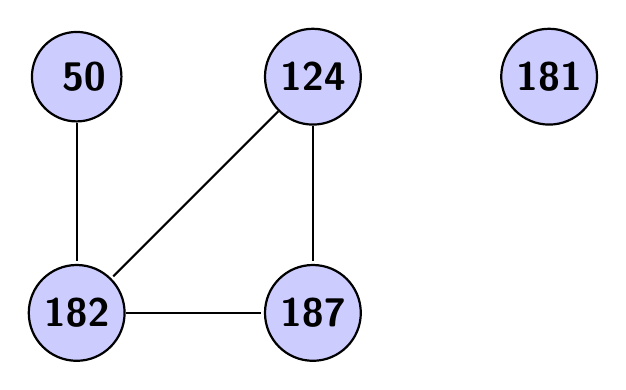
\begin{tikzpicture}[
            shorten >=1pt, auto, thick,
            node distance=2.5cm,
        main node/.style={circle,draw,fill=blue!20,font=\sffamily\Large\bfseries}
                                ]
          \node[main node] (a) at (0,0) {~50};
          \node[main node] (b) at (3,0) {124};
          \node[main node] (c) at (6,0) {181};
          \node[main node] (d) at (0,-3) {182};
          \node[main node] (e) at (3,-3) {187};
    
          \path[every node/.style={font=\sffamily\small}]
            (a) edge node {} (d)
            (b) edge node {} (d)
            (b) edge node {} (e)
            (d) edge node {} (e);
    \end{tikzpicture}
    \vspace{1em}
\else
    \vspace{12em}
    \pagebreak
\fi


\item Describe the standard backtracking search strategy to solve this problem. Write down a possible solution that you found using the strategy. 

\ifsol
    \textcolor{blue}{We can use backtracking to solve this problem. The domains dictate the possible next assignments, and we consider one assignment per step. We then check whether constraints are violated after each assignment. Once an incomplete end is reached, we backtrack up the search tree. In the following solution, we use the standard backtracking approach and assign the variables numerical order and professors in alphabetical order (You can look at the lecture notes for heuristics for picking the next unassigned variable, or to filter possible solutions which will solve this problem faster!):
    \begin{enumerate}
    \item We first pick $CS50: A$. There are no violated constraints.
    \item We now pick $CS124: B$. There are no violated constraints. The partial solution is $\{$CS50: A, CS124: B$\}$. 
    \item We now pick $CS181: A$. There are no violated constraints. The partial solution is $\{$CS50: A, CS124: B, CS181: A$\}$. 
    \item We now pick $CS182: A$. This violates the constraint $CS50 \neq CS182$. Therefore, we backtrack all the way to step (a) before we can address this.
    \item We now first pick $CS50: C$. There are no violated constraints. 
    \item We now pick $CS124: B$. There are no violated constraints. The partial solution is $\{$CS50: C, CS124: B$\}$. 
    \item We now pick $CS181: A$. There are no violated constraints. The partial solution is $\{$CS50: C, CS124: B, CS181: A$\}$. 
    \item We now pick $CS182: A$. There are no violated constraints. The partial solution is $\{$CS50: C, CS124: B, CS181: A, CS182: A$\}$. 
    \item We pick $CS187: B$. This does violate the constraint $CS124 \neq CS187$. We backtrack to step (h).
    \item We pick $CS187: C$. This does not violate a constraint. We are done. The final solution is $\{$CS50: C, CS124: B, CS181: A, CS182: A, CS187: C$\}$. 
    \end{enumerate}}
\else
    \vspace{35em}
\fi

\item Explain why it is a good heuristic to choose the variable that is most constrained but the value that is least constraining in a CSP search

\ifsol
    \textcolor{blue}{The reason that this heuristic is effective is that the variable with the least options is the hardest to satisfy, while the least constraining value leaves open the most options for other variables. This gives the highest chance of success. If we had done this above we would have finished the problem faster -- try it yourself!}
\else
    \vspace{5em}
\fi

\end{enumerate}

\end{document}